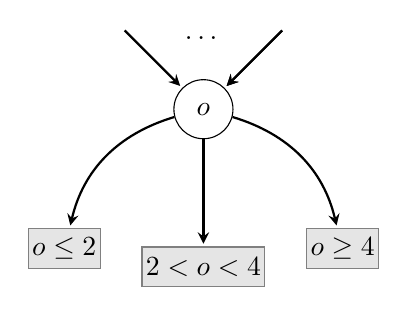
\begin{tikzpicture}
  [->, >=stealth, shorten >=1pt,auto,node distance=2cm,
    align=center,
    neuron/.style={%
      circle, draw, minimum size=0.75cm
    },
    bucket/.style={%
      rectangle,draw=black!50,fill=black!10,
      minimum size=5mm,inner sep=0.5mm
    },
  ]

  \node[neuron] (o) {$o$};
  \node[bucket] (b2) [below of=o, node distance=2cm] {$2 < o < 4$};
  \node[bucket] (b1) [below left of=o, node distance=2.5cm] {$o\leq2$};
  \node[bucket] (b3) [below right of=o, node distance=2.5cm] {$o\geq4$};

  \draw[->,thick] ++(-1,1) -- (o); 
  \draw[->,thick] ++(1,1) -- (o); 

  \draw[->,thick] ++(1,1) -- (o) node[above=0.75cm] {\dots};

  \path[->,thick]
  (o) edge [bend right] (b1)
      edge (b2)
      edge [bend left] (b3);

\end{tikzpicture}
